%%%%%%%%%%%%%%%%%%%%%%%%%%%%%%%%%%%%%%%%%%%%%%%%%%%%%%%%%%%%%%%%%%%%%%%%%%%%%%%
\chapter{The main question}
Here we want to answer the following question:
\begin{einr}
  Which information is needed to describe the Stokes structure of a
  (unramified) \textbf{multileveled} meromorphic connection?
\end{einr}
To be more precise: we are interested in the representation of an element from
$\prod_{\theta\in\A}\Sto_\theta(A^0)$ and how the information about the
different levels is stored.

\begin{comment}
  Ideas:
  \begin{enumerate}
    \item see algorithm~\cite[II.3.4]{Loday1994}
    \item search in \cite{Loday2014}
    \item generalize the ideas from \cite{boalch,thboalch}.
  \end{enumerate}
\end{comment}

\begin{comment}
  %%%%%%%%%%%%%%%%%%%%%%%%%%%%%%%%%%%%%%%%%%%%%%%%%%%%%%%%%%%%%%%%%%%%%%%%%%%%%%%
  \subsection{The single-level case}
  \marginnote{\cite{boalch,thboalch}}
  Here we will look at the case, when $\cK=\{k\}$ \comm{and when the connection
  is \textbf{simple}\footnote{\textbf{simple} means that all $q_i$'s are
  different.}}

  One can view the anti-Stokes directions as the directions, which help to
  distinguish between the elements of $\cQ_{[A^0]}$, since they mark the
  directions, where the differences of two such elements \TODO{}

  In this case has the set $\A$ a $\frac{\pi}{k}$-rotational symmetry (cf.\
  remark~\ref{rem:rotationalSymPrime}).
  This means, that in every arc of width $\frac{\pi}{k}$ are
\end{comment}

%%%%%%%%%%%%%%%%%%%%%%%%%%%%%%%%%%%%%%%%%%%%%%%%%%%%%%%%%%%%%%%%%%%%%%%%%%%%%%%
\begin{figure}[!htbp] %{{{
  \centering
  \begin{subfigure}[b]{0.33\textwidth}
    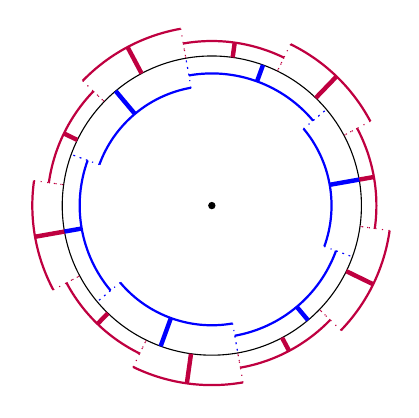
\begin{tikzpicture}[scale=1.9]
      \node (zero) at (0,0) {};
      \draw (zero) circle (1cm);

      %%%%%%%%%%%%%%%%%%%%%%%%%%%%%%%%%%%%%%%%%%%%%%%%%%%%%%%%%%%%%%%%%%%%%%%%%%%
      %%%%  Purple
      \foreach \w in {10}
      % {\foreach \sep in {0,45,90,135,180,225,270,315}
      {\foreach \sep in {0,36,72,108,144,180,216,252,288,324}
       {%\draw[thick,purple] (0,0) -- +({cos( \w + \sep )},{sin( \w + \sep )});

        \pgfmathsetmacro\r{{1.1 + mod(\w,10)/100 + mod(\sep,72)/360}}
        \draw[ultra thick,purple] ({cos( \w + \sep )},{sin( \w + \sep )})
          -- ({cos( \w + \sep) * \r},{sin( \w + \sep) * \r});

        \draw[thick,purple] ({cos( \w + \sep -18) * \r},{sin( \w + \sep -18) * \r})
          arc ({\w + \sep - 18}:{\w + \sep +18}:\r);

        \draw[dotted,purple] ({cos( \w + \sep -18) * \r},{sin( \w + \sep -18) * \r})
          -- ({cos( \w + \sep -18) * 1},{sin( \w + \sep -18) * 1});
        \draw[dotted,purple] ({cos( \w + \sep +18) * \r},{sin( \w + \sep +18) * \r})
          -- ({cos( \w + \sep +18) * 1},{sin( \w + \sep +18) * 1});
        }};

      %%%%%%%%%%%%%%%%%%%%%%%%%%%%%%%%%%%%%%%%%%%%%%%%%%%%%%%%%%%%%%%%%%%%%%%%%%%
      %%%%  Blue
      \foreach \w in {10}
      {\foreach \sep in {0,60,120,180,240,300}
       {%\draw[blue] (0,0) -- +({cos( \w + \sep ) * 0.9},{sin( \w + \sep ) * 0.9});
     
        \pgfmathsetmacro\r{{0.8 + mod(\w,10)/100 + mod(\sep,120)/720}}

        \draw[ultra thick,blue] ({cos( \w + \sep )},{sin( \w + \sep )})
          -- ({cos( \w + \sep) * \r},{sin( \w + \sep) * \r});
        \draw[thick,blue] ({cos( \w + \sep -30) * \r},{sin( \w + \sep -30) * \r})
          arc ({\w + \sep - 30}:{\w + \sep +30}:\r);


        \draw[dotted,blue] ({cos( \w + \sep -30) * \r},{sin( \w + \sep -30) * \r})
          -- ({cos( \w + \sep -30) * 1},{sin( \w + \sep -30) * 1});
        \draw[dotted,blue] ({cos( \w + \sep +30) * \r},{sin( \w + \sep +30) * \r})
          -- ({cos( \w + \sep +30) * 1},{sin( \w + \sep +30) * 1});
      }};


      % %%%%%%%%%%%%%%%%%%%%%%%%%%%%%%%%%%%%%%%%%%%%%%%%%%%%%%%%%%%%%%%%%%%%%%%%%%%
      % %%%%  Green
      % \foreach \w in {10}
      % {\foreach \sep in {0,90,180,270}
      %  {%\draw[green!60!black] (0,0) -- +({cos( \w + \sep ) * 0.8},{sin( \w + \sep) * 0.8});
     
      %   \pgfmathsetmacro\r{{0.8 + mod(\w,10)/100 + mod(\sep,180)/900}}

      %   \draw[ultra thick,green!60!black] ({cos( \w + \sep )},{sin( \w + \sep )})
      %     -- ({cos( \w + \sep) * \r},{sin( \w + \sep) * \r});
      %   \draw[thick,green!60!black] ({cos( \w + \sep -45) * \r},{sin( \w + \sep -45) * \r})
      %     arc ({\w + \sep - 45}:{\w + \sep +45}:\r);


      %   \draw[dotted,green!60!black] ({cos( \w + \sep -45) * \r},{sin( \w + \sep -45) * \r})
      %     -- ({cos( \w + \sep -45) * 1},{sin( \w + \sep -45) * 1});
      %   \draw[dotted,green!60!black] ({cos( \w + \sep +45) * \r},{sin( \w + \sep +45) * \r})
      %     -- ({cos( \w + \sep +45) * 1},{sin( \w + \sep +45) * 1});
     
      % }};

      \fill[white] (zero) circle (1.5pt);
      \fill (zero) circle (.7pt);
    \end{tikzpicture}
    \caption{$\cK=\{\textcolor{purple}{5},\textcolor{blue}{3}\}$}
  \end{subfigure}%
  \begin{subfigure}[b]{0.33\textwidth}
    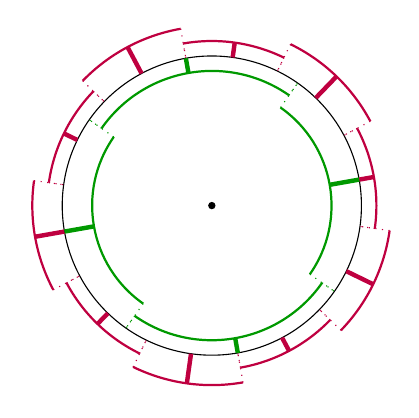
\begin{tikzpicture}[scale=1.9]
      \node (zero) at (0,0) {};
      \draw (zero) circle (1cm);

      %%%%%%%%%%%%%%%%%%%%%%%%%%%%%%%%%%%%%%%%%%%%%%%%%%%%%%%%%%%%%%%%%%%%%%%%%%%
      %%%%  Purple
      \foreach \w in {10}
      % {\foreach \sep in {0,45,90,135,180,225,270,315}
      {\foreach \sep in {0,36,72,108,144,180,216,252,288,324}
       {%\draw[thick,purple] (0,0) -- +({cos( \w + \sep )},{sin( \w + \sep )});

        \pgfmathsetmacro\r{{1.1 + mod(\w,10)/100 + mod(\sep,72)/360}}
        \draw[ultra thick,purple] ({cos( \w + \sep )},{sin( \w + \sep )})
          -- ({cos( \w + \sep) * \r},{sin( \w + \sep) * \r});

        \draw[thick,purple] ({cos( \w + \sep -18) * \r},{sin( \w + \sep -18) * \r})
          arc ({\w + \sep - 18}:{\w + \sep +18}:\r);

        \draw[dotted,purple] ({cos( \w + \sep -18) * \r},{sin( \w + \sep -18) * \r})
          -- ({cos( \w + \sep -18) * 1},{sin( \w + \sep -18) * 1});
        \draw[dotted,purple] ({cos( \w + \sep +18) * \r},{sin( \w + \sep +18) * \r})
          -- ({cos( \w + \sep +18) * 1},{sin( \w + \sep +18) * 1});
        }};

      % %%%%%%%%%%%%%%%%%%%%%%%%%%%%%%%%%%%%%%%%%%%%%%%%%%%%%%%%%%%%%%%%%%%%%%%%%%%
      % %%%%  Blue
      % \foreach \w in {10}
      % {\foreach \sep in {0,60,120,180,240,300}
      %  {%\draw[blue] (0,0) -- +({cos( \w + \sep ) * 0.9},{sin( \w + \sep ) * 0.9});
     
      %   \pgfmathsetmacro\r{{0.8 + mod(\w,10)/100 + mod(\sep,120)/720}}

      %   \draw[ultra thick,blue] ({cos( \w + \sep )},{sin( \w + \sep )})
      %     -- ({cos( \w + \sep) * \r},{sin( \w + \sep) * \r});
      %   \draw[thick,blue] ({cos( \w + \sep -30) * \r},{sin( \w + \sep -30) * \r})
      %     arc ({\w + \sep - 30}:{\w + \sep +30}:\r);


      %   \draw[dotted,blue] ({cos( \w + \sep -30) * \r},{sin( \w + \sep -30) * \r})
      %     -- ({cos( \w + \sep -30) * 1},{sin( \w + \sep -30) * 1});
      %   \draw[dotted,blue] ({cos( \w + \sep +30) * \r},{sin( \w + \sep +30) * \r})
      %     -- ({cos( \w + \sep +30) * 1},{sin( \w + \sep +30) * 1});
      % }};


      %%%%%%%%%%%%%%%%%%%%%%%%%%%%%%%%%%%%%%%%%%%%%%%%%%%%%%%%%%%%%%%%%%%%%%%%%%%
      %%%%  Green
      \foreach \w in {10}
      {\foreach \sep in {0,90,180,270}
       {%\draw[green!60!black] (0,0) -- +({cos( \w + \sep ) * 0.8},{sin( \w + \sep) * 0.8});
     
        \pgfmathsetmacro\r{{0.8 + mod(\w,10)/100 + mod(\sep,180)/900}}

        \draw[ultra thick,green!60!black] ({cos( \w + \sep )},{sin( \w + \sep )})
          -- ({cos( \w + \sep) * \r},{sin( \w + \sep) * \r});
        \draw[thick,green!60!black] ({cos( \w + \sep -45) * \r},{sin( \w + \sep -45) * \r})
          arc ({\w + \sep - 45}:{\w + \sep +45}:\r);


        \draw[dotted,green!60!black] ({cos( \w + \sep -45) * \r},{sin( \w + \sep -45) * \r})
          -- ({cos( \w + \sep -45) * 1},{sin( \w + \sep -45) * 1});
        \draw[dotted,green!60!black] ({cos( \w + \sep +45) * \r},{sin( \w + \sep +45) * \r})
          -- ({cos( \w + \sep +45) * 1},{sin( \w + \sep +45) * 1});
     
      }};

      \fill[white] (zero) circle (1.5pt);
      \fill (zero) circle (.7pt);
    \end{tikzpicture}
    \caption{$\cK=\{\textcolor{purple}{5},\textcolor{green!60!black}{2}\}$}
  \end{subfigure}%
  \begin{subfigure}[b]{0.33\textwidth}
    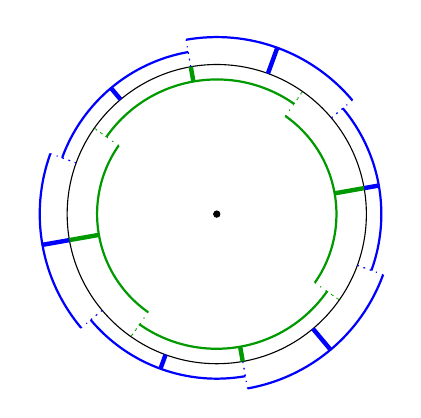
\begin{tikzpicture}[scale=1.9]
      \node (zero) at (0,0) {};
      \draw (zero) circle (1cm);

      %%%%%%%%%%%%%%%%%%%%%%%%%%%%%%%%%%%%%%%%%%%%%%%%%%%%%%%%%%%%%%%%%%%%%%%%%%%
      %%%%  Purple
      % \foreach \w in {10}
      % % {\foreach \sep in {0,45,90,135,180,225,270,315}
      % {\foreach \sep in {0,36,72,108,144,180,216,252,288,324}
      %  {%\draw[thick,purple] (0,0) -- +({cos( \w + \sep )},{sin( \w + \sep )});

      %   \pgfmathsetmacro\r{{1.1 + mod(\w,10)/100 + mod(\sep,72)/360}}
      %   \draw[ultra thick,purple] ({cos( \w + \sep )},{sin( \w + \sep )})
      %     -- ({cos( \w + \sep) * \r},{sin( \w + \sep) * \r});

      %   \draw[thick,purple] ({cos( \w + \sep -18) * \r},{sin( \w + \sep -18) * \r})
      %     arc ({\w + \sep - 18}:{\w + \sep +18}:\r);

      %   \draw[dotted,purple] ({cos( \w + \sep -18) * \r},{sin( \w + \sep -18) * \r})
      %     -- ({cos( \w + \sep -18) * 1},{sin( \w + \sep -18) * 1});
      %   \draw[dotted,purple] ({cos( \w + \sep +18) * \r},{sin( \w + \sep +18) * \r})
      %     -- ({cos( \w + \sep +18) * 1},{sin( \w + \sep +18) * 1});
      %   }};

      %%%%%%%%%%%%%%%%%%%%%%%%%%%%%%%%%%%%%%%%%%%%%%%%%%%%%%%%%%%%%%%%%%%%%%%%%%%
      %%%%  Blue
      \foreach \w in {10}
      {\foreach \sep in {0,60,120,180,240,300}
       {%\draw[blue] (0,0) -- +({cos( \w + \sep ) * 0.9},{sin( \w + \sep ) * 0.9});
     
        \pgfmathsetmacro\r{{1.1 + mod(\w,10)/100 + mod(\sep,120)/720}}

        \draw[ultra thick,blue] ({cos( \w + \sep )},{sin( \w + \sep )})
          -- ({cos( \w + \sep) * \r},{sin( \w + \sep) * \r});
        \draw[thick,blue] ({cos( \w + \sep -30) * \r},{sin( \w + \sep -30) * \r})
          arc ({\w + \sep - 30}:{\w + \sep +30}:\r);


        \draw[dotted,blue] ({cos( \w + \sep -30) * \r},{sin( \w + \sep -30) * \r})
          -- ({cos( \w + \sep -30) * 1},{sin( \w + \sep -30) * 1});
        \draw[dotted,blue] ({cos( \w + \sep +30) * \r},{sin( \w + \sep +30) * \r})
          -- ({cos( \w + \sep +30) * 1},{sin( \w + \sep +30) * 1});
      }};


      %%%%%%%%%%%%%%%%%%%%%%%%%%%%%%%%%%%%%%%%%%%%%%%%%%%%%%%%%%%%%%%%%%%%%%%%%%%
      %%%%  Green
      \foreach \w in {10}
      {\foreach \sep in {0,90,180,270}
       {%\draw[green!60!black] (0,0) -- +({cos( \w + \sep ) * 0.8},{sin( \w + \sep) * 0.8});
     
        \pgfmathsetmacro\r{{0.8 + mod(\w,10)/100 + mod(\sep,180)/900}}

        \draw[ultra thick,green!60!black] ({cos( \w + \sep )},{sin( \w + \sep )})
          -- ({cos( \w + \sep) * \r},{sin( \w + \sep) * \r});
        \draw[thick,green!60!black] ({cos( \w + \sep -45) * \r},{sin( \w + \sep -45) * \r})
          arc ({\w + \sep - 45}:{\w + \sep +45}:\r);


        \draw[dotted,green!60!black] ({cos( \w + \sep -45) * \r},{sin( \w + \sep -45) * \r})
          -- ({cos( \w + \sep -45) * 1},{sin( \w + \sep -45) * 1});
        \draw[dotted,green!60!black] ({cos( \w + \sep +45) * \r},{sin( \w + \sep +45) * \r})
          -- ({cos( \w + \sep +45) * 1},{sin( \w + \sep +45) * 1});
     
      }};

      \fill[white] (zero) circle (1.5pt);
      \fill (zero) circle (.7pt);
    \end{tikzpicture}
    \caption{$\cK=\{\textcolor{blue}{3},\textcolor{green!60!black}{2}\}$}
  \end{subfigure}
  \caption{Ideas for examples with two levels.}
\end{figure} %}}}

%%%%%%%%%%%%%%%%%%%%%%%%%%%%%%%%%%%%%%%%%%%%%%%%%%%%%%%%%%%%%%%%%%%%%%%%%%%%%%%
\section{Building our example}
We want to have a unramified connection with more than one level. Two levels
might be enough. 

Let us start by defining the determining polynomials
\[
  q_j(t^{-1})=\frac{a_j}{t^{l_j}}+h_j
\]
where 
\begin{itemize}
  \item $a_j\in\C\backslash\{0\}$,
  \item $l_j\in\Z$ (since we want to be unramified) and
  \item $h_j\in o(t^{-k})$ \TODO[not enough information]
\end{itemize}
thus our system has the levels $\cK=\{k_1<k_2<\cdots<k_r\}=\{l_1,\dots,l_n\}$.
We then construct the connection matrix by
\[
  A^0=e^{Q(t^{-1})}+t^L
\]
where
\begin{itemize}
  \item $Q(t^{-1})=\diag(q_1(t^{-1}),q_2(t^{-1}),\dots,q_n(t^{-1}))$
    and
  \item $L$ is konstant\comm{~and in jordan normalform/diagonal}.
\end{itemize}

\begin{lem}
  The matrix $\cY_0:=t^Le^{Q(t^{-1})}$ is then a fundamental solution of
  $[A^0]$.
\end{lem}
\begin{proof}
  It is sufficient to show that $\cY\in G(\!\{t\}\!)$ and
  \[
    \frac{d}{dt}\cY_0=A\cY_0 \,.
  \]
  \rewrite{The right hand side}
  \begin{align*}
    A\cY_0
    &=\left(e^{Q(t^{-1})}+t^L\right)t^Le^{Q(t^{-1})}
  \\&=e^{Q(t^{-1})}t^Le^{Q(t^{-1})}+t^Lt^Le^{Q(t^{-1})}
  \end{align*}
  and \rewrite{the left hand side}
  \begin{align*}
    \frac{d}{dt}\cY_0
    &=\frac{d}{dt}\left(t^Le^{Q(t^{-1})}\right)
  \\&=\frac{d}{dt}\left(e^{L\ln t}e^{Q(t^{-1})}\right)
  \\&=\frac{d}{dt}e^{L\ln t}e^{Q(t^{-1})}+e^{L\ln t}\frac{d}{dt}e^{Q(t^{-1})}
  \end{align*}
  \TODO{}
\end{proof}






